\chapter{Further Properties of Homomorphisms}
Earlier in this book, we introduced homomorphisms and isomorphisms, special types of maps that transform elements of one group to another. We look at more properties of such maps in this chapter and describe the uses of these new properties.

\section{Image of a Homomorphism}
As a homomorphism is a mapping between two groups, it is worthy to look at the \textbf{image} of the homomorphism.
\begin{definition}
    The \textbf{image}\index{homomorphism!image} (or \textbf{range}\index{homomorphism!range}) of a homomorphism $\phi: G \to H$ is the set
    \[
        \im\phi = \{\phi(g) \vert g \in G\}.
    \]
\end{definition}
\begin{remark}
    Some authors (e.g. \cite{libretexts_im-and-ker}) will use the notation $\phi(G)$ for the image of $\phi$. The alternate notation $\mathrm{Im}\;\phi$ may also be used (e.g. by \cite{clark_1984, hungerford_1980}).
\end{remark}

\begin{example}
    Consider the homomorphism $f: \mathbb{Z} \to \mathbb{Z}, x \mapsto 0$. Clearly, all possible values of $x$ maps to 0, so $\im f = \{0\}$.
\end{example}
\begin{example}
    The homomorphism $f: \mathbb{R} \to \mathbb{R}$ where $f(x) = |x|$ has an image of $\{x \in \mathbb{R} \vert x \geq 0\}$, i.e. all non-negative real numbers.
\end{example}

We note that the image of a homomorphism is a subgroup of the codomain $H$.
\begin{proposition}\label{prop-image-is-subgroup-of-codomain}
    Let $\phi: G \to H$ be a homomorphism. Then $\im\phi \leq H$.
\end{proposition}
\begin{proof}
    We consider the subgroup test.
    
    Note that $\phi(e_G) = e_H \in \im\phi$, where $e_G$ and $e_H$ are the identities of $G$ and $H$ respectively.
    
    Now suppose $h_1$ and $h_2$ are in the image of $\phi$, meaning that there exists $g_1$ and $g_2$ such that $\phi(g_1) = h_1$ and $\phi(g_2) = h_2$. Note that $\phi(g_2^{-1}) = h_2^{-1}$ by homomorphism property. Hence $\phi(g_1g_2^{-1}) = h_1h_2^{-1} \in \im\phi$.

    Therefore, by subgroup test, $\im\phi \leq H$.
\end{proof}

\begin{exercise}
    Consider the map $\phi: \mathbb{Z}_3 \to \mathbb{Z}_6, n \mapsto 2n$. Determine whether $\phi$ is a homomorphism and, if so, find its image.
\end{exercise}

\section{Kernel of a Homomorphism}
\begin{definition}
    The \textbf{kernel}\index{homomorphism!kernel} of a homomorphism $\phi: G \to H$ is the set
    \[
        \ker\phi = \{x \in G \vert \phi(x) = e_H\}
    \]
    where $e_H$ is the identity in $H$.
\end{definition}
Basically, the kernel of $\phi$ is the set of elements in $G$ which map to the identity in $H$.

\begin{remark}
    Some authors (e.g. \cite{libretexts_im-and-ker}) will use the notation $\phi^{-1}(e_H)$ for the kernel of $\phi$. The alternate notation $\mathrm{Ker}\;\phi$ may also be used by some authors (e.g. \cite{clark_1984, hungerford_1980}).
\end{remark}

\begin{example}
    Let the groups $G = (\mathbb{Z}^2, (+, +))$ and $H = (\mathbb{Z}, +)$. Let the map $\phi: G \to H, (a, b) \mapsto a+b$. Then, $(a, b) \in \ker\phi$ if $\phi((a,b)) = 0$. This means that $a+b = 0$, implying $ b = -a$. Hence the kernel of $\phi$ is $\{(a, -a) \vert a \in \mathbb{Z}\}$.
\end{example}

\begin{exercise}
    Let $i$ be the imaginary unit, that is $i^2 = -1$. Let the group $G$ be the integers under addition and $H = \langle i \rangle$ be under multiplication. Let the map $\phi: G \to H, n \mapsto i^n$.  Show that $\phi$ is a homomorphism and hence find $\ker\phi$.
\end{exercise}

We observe that the kernel of $\phi$ is a subgroup of $G$. It is, in fact, a \textit{normal} subgroup of $G$.
\begin{proposition}\label{prop-kernel-is-normal-subgroup-of-domain}
    Let $\phi: G \to H$ be a homomorphism. Then $\ker\phi \unlhd G$.
\end{proposition}
\begin{proof}
    We will first show $\ker\phi\leq G$. Clearly $e_G \in \ker\phi$ since $\phi(e_G) = e_H$, so $\ker\phi$ is non-empty. Now let $x, y \in \ker\phi$. This means that $\phi(x) = \phi(y) = e_H$. Note
    \begin{align*}
        \phi(xy^{-1}) &= \phi(x)\left(\phi(y)\right)^{-1}\\
        &= e_H(e_H)^{-1}\\
        &= e_H
    \end{align*}
    which means that $xy^{-1}\in\ker\phi$. By subgroup test, $\ker\phi\leq G$.

    Now we prove normality. Let $x \in G$ and $n \in \ker\phi$. We need to show that $xnx^{-1}\in\ker\phi$ to prove normality. Observe that
    \begin{align*}
        \phi(xnx^{-1}) &= \phi(x)\phi(n)\phi(x^{-1})\\
        &= \phi(x)e_H\phi(x)^{-1} & (n \in \ker\phi)\\
        &= \phi(x)\phi(x)^{-1}\\
        &= e_H,
    \end{align*}
    which means that $xnx^{-1} \in \ker\phi$. Hence, $\ker\phi \unlhd G$.
\end{proof}

\begin{exercise}\label{exercise-trivial-kernel-means-injective}
    Prove that a homomorphism $\phi:G\to H$ is injective if and only if $\ker \phi$ is trivial, i.e. $\ker \phi = \{e_G\}$.
\end{exercise}

\section{The Fundamental Homomorphism Theorem}
We are now ready to tackle the three most important theorems regarding homomorphisms. We first state the \textbf{Fundamental Homomorphism Theorem}, which is also sometimes called the \textbf{First Isomorphism Theorem}.
\begin{theorem}[Fundamental Homomorphism Theorem]\label{thrm-isomorphism-1}\index{Fundamental Homomorphism Theorem}\index{Isomorphism Theorem!First}
    Let $G$ and $H$ be groups. Let $\phi: G \to H$ be a homomorphism, and let $\pi: G \to G/\ker\phi$ where $g\mapsto g\ker\phi$ be the natural surjective homomorphism. Then there exists a unique isomorphism $\psi: G/\ker\phi \to \im\phi$ such that $\psi\pi = \phi$.
\end{theorem}
\begin{remark}
    Equivalently, the Fundamental Homomorphism Theorem states that
    \[
        G/\ker\phi \cong \im\phi
    \]
    for any homomorphism $\phi$.
\end{remark}

We include the commutativity diagram of the homomorphisms stated to aid clarity:

\begin{figure}[h]
    \centering
    \fbox{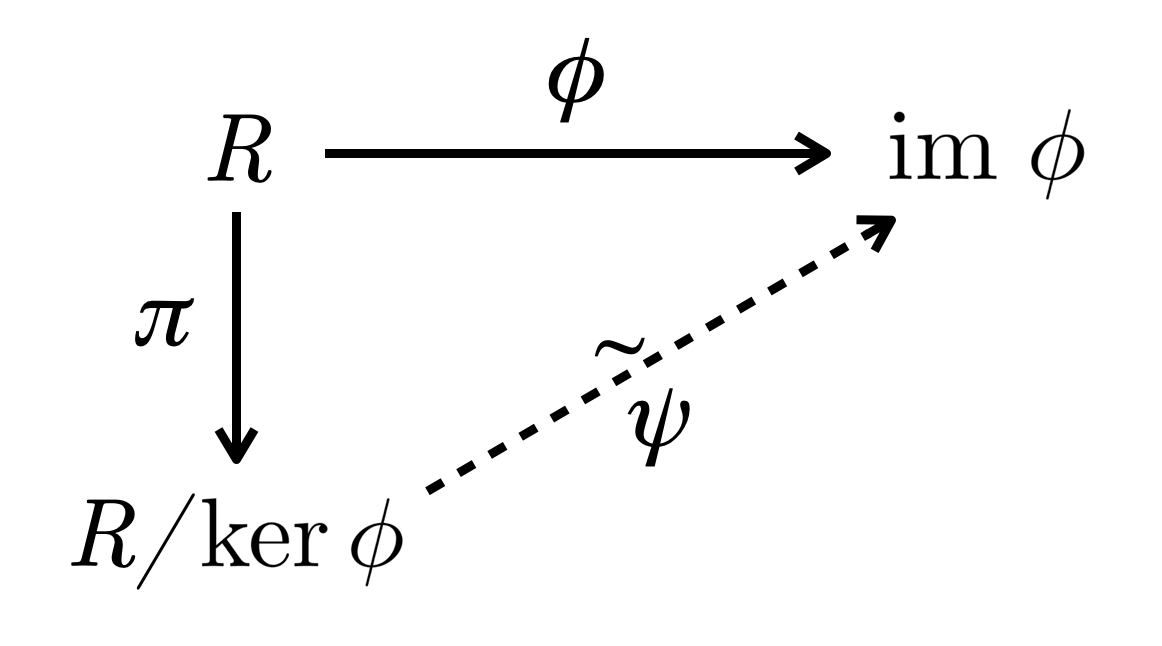
\includegraphics[width=0.25\textwidth]{further-homomorphisms/iso-1-comm-diagram.png}}
    \caption{Commutativity Diagram for \myreffigures{thrm-isomorphism-1}}
\end{figure}

In the diagram, $\phi$ sends elements from $G$ to $\im\phi$ and $\pi$ sends elements from $G$ to $G/\ker\phi$. Then the map $\psi$ is a unique map that sends elements from $G/\ker\phi$ to the image of $\phi$.

\begin{proof}[Proof (cf. {\cite[p.~250, Theorem 2]{cohn_1982}})]
    We know by \myref{prop-image-is-subgroup-of-codomain} that $\im\phi \leq H$. Let $\psi: G/\ker\phi \to \im\phi$ such that $\psi(x\ker\phi) = \phi(x)$. We need to check that $\psi$ is a well-defined isomorphism.
    \begin{itemize}
        \item \textbf{Well-defined}: Suppose $x\ker\phi = y\ker\phi$ where $x, y \in G$. Then $xy^{-1} \in \ker\phi$ by Coset Equality (\myref{lemma-coset-equality}), statements 1 and 5. This means that $\phi(xy^{-1}) = e_H$ by definition of the kernel. Note $\phi(xy^{-1}) = \phi(x)\left(\phi(y)\right)^{-1}$, so $\phi(x)\left(\phi(y)\right)^{-1} = e_H$. Hence $\phi(x) = \phi(y)$. Thus,
        \[
            \psi(x\ker\phi) = \phi(x) = \phi(y) = \psi(y\ker\phi)
        \]
        so $\psi$ is well-defined.

        \item \textbf{Homomorphism}: Note that
        \begin{align*}
            \psi((x\ker\phi)(y\ker\phi)) &= \psi((xy)\ker\phi)\\
            &= \phi(xy)\\
            &= \phi(x)\phi(y)\\
            &= \psi(x\ker\phi)\psi(y\ker\phi)
        \end{align*}
        so $\psi$ is a homomorphism.
        \item \textbf{Injective}: By \myref{exercise-trivial-kernel-means-injective}, we check that $\psi$ is injective by showing that $\ker\psi$ is trivial, i.e. $\ker\psi = \{\ker\phi\}$.

        Suppose $x\ker\phi\in\ker\psi$. Then $\psi(x\ker\phi) = e_H$ by definition of kernel. Hence $\phi(x) = e_H$ by definition of $\psi$, which means $x \in \ker\phi$ by definition of kernel. Thus $x\ker\phi = \ker\phi$ by Element in Coset (\myref{corollary-equivalence-of-element-in-coset}). Therefore $\psi$ is injective.

        \item \textbf{Surjective}: Suppose $y$ is in the image of $\phi$, meaning there exists a $x \in G$ such that $\phi(x) = y$. Note that $\psi(x\ker\phi) = \phi(x) = y$. Thus $\psi$ is surjective.
    \end{itemize}
    Thus $\psi$ is a well-defined isomorphism.

    We now check that $\psi$ satisfies the requirement that $\psi\pi = \phi$. Let $x \in G$. Note that $\pi(x) = x\ker\phi$, and
    \[
        \psi\pi(x) = \psi(x\ker\phi) = \phi(x)
    \]
    for all $x \in G$, so $\psi\pi = \phi$.

    Finally we show that $\psi$ is unique. Suppose $f: G/\ker\phi \to \im\phi$ is an isomorphism satisfying $f\pi=\phi$. Take $x\ker\phi \in G/\ker\phi$. Note that
    \begin{align*}
        f(x\ker\phi) &= f(\pi(x))\\
        &= (f\pi)(x)\\
        &= \phi(x)\\
        &= (\psi\pi)(x)\\
        &= \psi(\pi(x))\\
        &= \psi(x\ker\phi)
    \end{align*}
    for all $x \in G$, meaning that $f = \psi$. Therefore $\psi$ is unique.

    Hence, $\psi$ is a unique isomorphism satisfying $\psi\pi = \phi$.
\end{proof}

\begin{example}
    Let $R = \{x \in \mathbb{R} \vert x > 0\}$, $G = \{x \in \mathbb{R} \vert x \neq 0\}$, and $H = \{1, -1\}$ be groups under multiplication. We show $G / H \cong R$.

    Consider the map $\phi: G \to R$ where $x \mapsto |x|$. We show that $\phi$ is a homomorphism, then find the image of $\phi$, and finally find its kernel.

    \newpage

    \begin{itemize}
        \item \textbf{Homomorphism}: $\phi$ is a homomorphism since $\phi(xy) = |xy| = |x||y| = \phi(x)\phi(y)$.
        \item \textbf{Image}: We find the image of $\phi$.
        \begin{align*}
            \im\phi &= \{\phi(x) \vert x \in G\}\\
            &= \{|x| \vert x \neq 0\}\\
            &= \{x \in \mathbb{R} \vert x > 0\} & (\text{by definition of } |x|)\\
            &= R
        \end{align*}
        which actually means that $\phi$ is surjective.
        \item \textbf{Kernel}: We find the kernel of $\phi$.
        \begin{align*}
            \ker\phi &= \{x \in G \vert \phi(x) = 1\} & (1 \text{ is the identity in } R)\\
            &= \{x \in G \vert |x| = 1\}\\
            &= \{1, -1\}\\
            &= H
        \end{align*}
    \end{itemize}
    Thus $G/H \cong R$ by the Fundamental Homomorphism Theorem (\myref{thrm-isomorphism-1}).
\end{example}

\begin{exercise}
    Let $\phi: G \to H$ be a homomorphism between finite groups $G$ and $H$. Prove that
    \[
        |G| = |\im \phi|\times|\ker \phi|.
    \]
\end{exercise}

\section{The Diamond Isomorphism Theorem}
We now look at the next theorem, called the \textbf{Diamond Isomorphism Theorem} or the \textbf{Second Isomorphism Theorem}.
\begin{theorem}[Diamond Isomorphism Theorem]\label{thrm-isomorphism-2}\index{Diamond Isomorphism Theorem}\index{Isomorphism Theorem!Second}
    Let $G$ be a group and let $H$ and $K$ be subgroups of $G$. Then
    \begin{enumerate}
        \item $H \cap K \leq H$; and
        \item $H \leq HK$.
    \end{enumerate}
    Furthermore, if $N \unlhd G$, then
    \begin{enumerate}[start=3]
        \item $HN \leq G$;
        \item $H \cap N \unlhd H$;
        \item $N \unlhd HN$; and
        \item $H / (H\cap N) \cong HN / N$.
    \end{enumerate}
\end{theorem}

\newpage

We can capture the overall relationships of the subgroups of $G$ using a \textbf{subgroup lattice}.
\begin{figure}[h]
    \centering
    \fbox{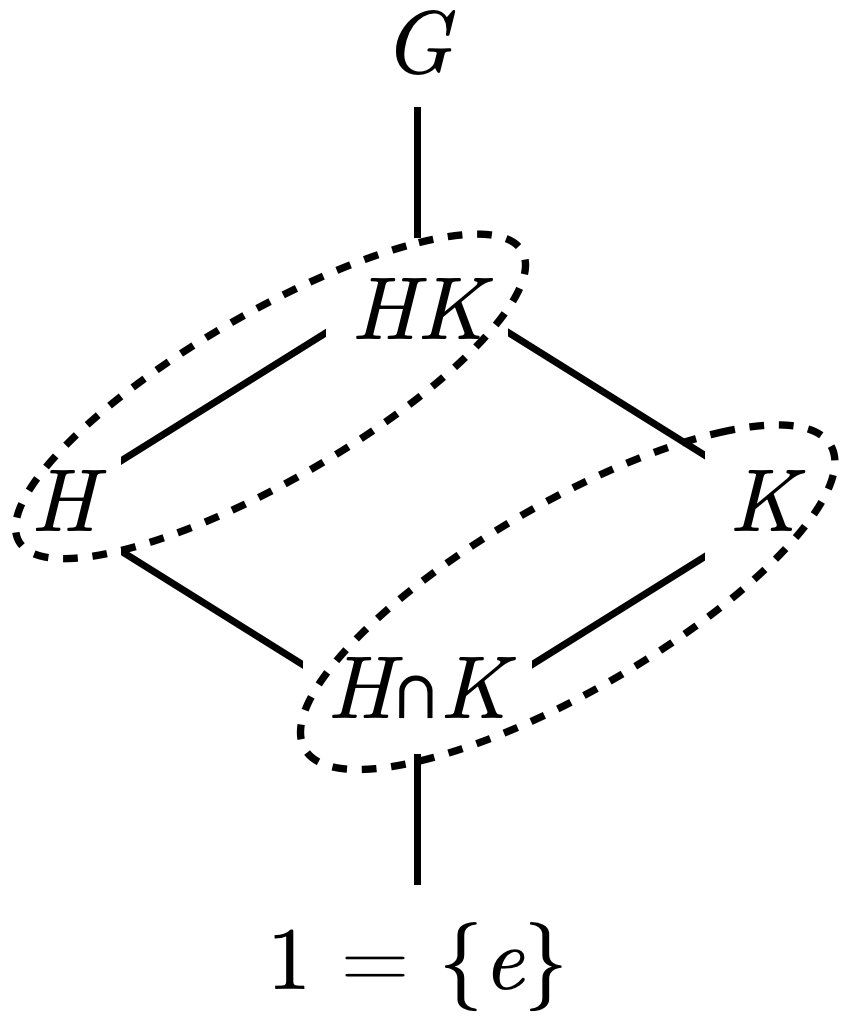
\includegraphics[width=0.25\textwidth]{further-homomorphisms/iso-2-subgroup-diagram.png}}
    \caption{Subgroup Lattice for \myreffigures{thrm-isomorphism-2}}
\end{figure}

We only show subgroups that we care about in the diagram. The group $G$ has a (direct) subgroup $HK$; $HK$ has subgroups $H$ and $K$; and $H$ and $K$ has a common subgroup $H\cap K$. The dotted quotient groups are isomorphic to each other if $H \unlhd G$.

\begin{proof}
    We prove each statement in sequence.

    \begin{enumerate}
        \item Clearly $e_G \in H$ and $e_G \in K$ so $e_G \in H \cap K$. Now take $x, y \in H \cap K$, meaning $x, y \in H$ and $x, y \in K$. Since $H, K \leq G$ so $xy^{-1} \in H$ and $xy^{-1} \in K$. Thus $xy^{-1} \in H \cap K$. By the subgroup test, this means that $H \cap K \leq H$.
        
        \item Note that $H = \{he_G \vert h \in H\} \subseteq \{hk \vert h \in H, k \in K\} = HK$, and $H$ is a group (as $H$ is a subgroup). Therefore $H \leq HK$.
        
        \item We note that, because $N$ is normal, hence $hN = Nh$ for all $h \in H \subseteq G$, meaning that $HN = NH$. Therefore by \myref{prop-subgroup-product-is-subgroup}, we have $HN \leq G$.

        \item We know $H \cap N \leq H$ by statement 1, so we only prove normality. Take $x \in H \cap N$. Since $H \leq G$, thus $x \in H \cap N \subseteq H$, meaning for all $g \in H$, $gxg^{-1} \in H$ (where we think of $g$ and $x$ as being in $H$). But since $x \in H \cap N \subseteq N$ and $N \unlhd G$, thus $gxg^{-1} \in N$ (where we think of $g \in H$ and $x \in N$). Therefore $H \cap N \unlhd H$.

        \item We know $N \leq HN$ by statement 2, so we only prove normality. Take $n \in N$ and $x \in HN$ such that $x = h_xn_x$. Then
        \begin{align*}
            xnx^{-1} &= (h_xn_x)n(h_xn_x)^{-1}\\
            &= (h_xn_x)n(n_x^{-1}h_x^{-1}) & (\text{Shoes and Socks})\\
            &= \underbrace{h_x}_{\text{In }G}\underbrace{n_xnn_x^{-1}}_{\text{In }N}\underbrace{h_x^{-1}}_{\text{In G}}\\
            &\in N
        \end{align*}
        since $N \unlhd G$. This proves that $N \unlhd HN$.

        \item This is the main result of this theorem. We define $\phi: H \to HN/N, h \mapsto hN$. We show that $\phi$ is a homomorphism and then find its image and kernel.
        \begin{itemize}
            \item \textbf{Homomorphism}:
            \[
                \phi(xy) = (xy)N = (xN)(yN) = \phi(x)\phi(y)    
            \]

            \item \textbf{Image}: We show that $\phi$ is surjective to show that $\im\phi = HN/N$. Suppose $x \in HN$, meaning $x = hn$ where $h \in H$ and $n \in N$. Thus $xN \in HN/N$, so
            \[
                xN = (hn)N = h(nN) = hN
            \]
            meaning $\phi(h) = hN = xN$. Hence we have found a pre-image of the coset $xN$, meaning $\phi$ is surjective. Thus $\im \phi = HN/N$.

            \item \textbf{Kernel}: We claim that $\ker\phi = H \cap N$.
            
            Note that $\ker\phi = \{h \in H \vert \phi(h) = eN = N\}$ by definition of kernel. This means that if $h \in \ker\phi$ then $\phi(h) = N$. Hence $\phi(h) = hN = N$, which means $h \in N$ by Element in Coset (\myref{corollary-equivalence-of-element-in-coset}). Thus, $h \in H$ and $h \in N$, meaning $h \in H \cap N$. Therefore $\ker \phi \subseteq H \cap N$.
    
            Now suppose $x \in H \cap N$. This means that $x \in N$ necessarily, implying $xN = N$. Thus $\phi(x) = N$ which quickly implies $x \in \ker\phi$. Therefore $H \cap N \subseteq \ker\phi$.
    
            Since $\ker \phi \subseteq H \cap N$ and  $H \cap N \subseteq \ker\phi$ therefore $\ker\phi = H\cap N$.
        \end{itemize}

        By the Fundamental Homomorphism Theorem (\myref{thrm-isomorphism-1}),
        \[
            H / \ker\phi \cong \im \phi,
        \]
        which means
        \[
            H/(H\cap N) \cong HN/N.
        \]
    \end{enumerate}
    This completes the proof of the theorem.
\end{proof}

\begin{corollary}\label{corollary-subgroup-product-is-normal-subgroup-if-subgroups-are-normal}
    Let $G$ be a group with proper subgroups $H$ and $K$. Then $HK \unlhd G$ if $H$ and $K$ are normal subgroups of $G$.
\end{corollary}
\begin{proof}
    Assume that $H, K \lhd G$. By the Diamond Isomorphism Theorem (\myref{thrm-isomorphism-2}), statement 3, we know that $HK \leq G$ since $H \lhd G$. We just need to prove normality. Suppose $hk \in HK$ and take $g \in G$. Then
    \begin{align*}
        g(hk)g^{-1} &= (gh)(kg^{-1})\\
        &= (hg)(g^{-1}k) & (\text{as } H, K \lhd G)\\
        &= h(gg^{-1})k\\
        &= hk \in HK
    \end{align*}
    which means that $HK \unlhd G$.
\end{proof}

We look at two examples using the Diamond Isomorphism Theorem.
\begin{example}
    We say a group $G$ is \textbf{metabelian}\index{metabelian} if and only if there exists $A \unlhd G$ such that $A$ and $G/A$ are both abelian. We will prove that any subgroup of a metabelian group is also metabelian.

    Let $H \leq G$. Then, by the Diamond Isomorphism Theorem (\myref{thrm-isomorphism-2}), we know $H \cap A \unlhd H$ (statement 4) and $H/(H \cap A) \cong HA / A$ (statement 6). We just need to prove that both $H \cap A$ and $H/(H \cap A)$ are abelian.
    \begin{itemize}
        \item Consider any two elements from $H \cap A$, say $x$ and $y$. Then $x \in A$ and $y \in A$, so $xy = yx$ as $A$ is abelian. Hence, elements from $H \cap A$ commute, meaning that $H \cap A$ is abelian.
        \item Consider $H/(H\cap A) \cong HA / A$. Note that $HA \leq G$ since $H \leq G$ and $A \leq G$. Thus, $HA / A \leq G / A$. Note that $G/A$ is abelian by definition of metabelian group. Hence, $H/(H \cap A)$ is also abelian.
    \end{itemize}
    Therefore, we have found a subgroup of $H$ (in particular $H \cap A$) such that both $H \cap A$ and $H/(H\cap A)$ are both abelian. Hence, $H$ is metabelian.
\end{example}

We look at another application of the Diamond Isomorphism Theorem, which has use in Number Theory.
\begin{example}
    We will prove that $\lcm(m,n)\times\gcd(m,n) = mn$ (\myref{prop-product-of-gcd-and-lcm}) by considering the Diamond Isomorphism Theorem. For brevity, let $d = \gcd(m,n)$ and $l = \lcm(m,n)$.

    Consider the groups $G = \mathbb{Z}$, $H = m\mathbb{Z}$, and $N = n\mathbb{Z}$ under addition. By Diamond Isomorphism Theorem (\myref{thrm-isomorphism-2}),
    \[
        m\mathbb{Z}/(m\mathbb{Z} \cap n\mathbb{Z}) \cong (m\mathbb{Z} + n\mathbb{Z})/(n\mathbb{Z}).
    \]

    Now $m\mathbb{Z} \cap n\mathbb{Z}$ is the set of integers that are both a multiple of $m$ and $n$. Hence, $m\mathbb{Z} \cap n\mathbb{Z} = \lcm(m,n)\mathbb{Z} = l\mathbb{Z}$. On the other hand, $m\mathbb{Z} + n\mathbb{Z}$ is the set of all integers of the form $mx+ny$ where $x$ and $y$ are integers. B\'{e}zout's lemma (\myref{lemma-bezout}) tells us that this set consists of the multiples of $\gcd(m,n)$, i.e. $m\mathbb{Z} + n\mathbb{Z} = \gcd(m,n)\mathbb{Z} = d\mathbb{Z}$. Hence,
    \[
        m\mathbb{Z}/(l\mathbb{Z}) \cong d\mathbb{Z}/(n\mathbb{Z}).
    \]

    We claim that $m\mathbb{Z} / (l\mathbb{Z}) \cong \mathbb{Z}_{\frac lm} \text{ and } d\mathbb{Z} / (n\mathbb{Z}) \cong \mathbb{Z}_{\frac nd}$. This is a specific case of \myref{problem-mZ/nZ-isomorphic-to-Zn/m} which we have left as a problem for later. Hence,
    \[
    \mathbb{Z}_{\frac lm} \cong m\mathbb{Z}/(l\mathbb{Z}) \cong d\mathbb{Z}/(n\mathbb{Z}) \cong \mathbb{Z}_{\frac nd},
    \]
    which means that $\mathbb{Z}_{\frac lm} \cong \mathbb{Z}_{\frac nd}$. We can now finally take orders on both sides:
    \[
        \frac{l}{m} = \frac{n}{d},
    \]
    which means that $ld = mn$. Hence, $\lcm(m,n)\times\gcd(m,n) = mn$.
\end{example}

\begin{exercise}\label{exercise-order-of-subgroup-product}
    Let $G$ be a finite group, $H \leq G$, and $N \lhd G$. Prove that
    \[
        |HN| = \frac{|H||N|}{|H \cap N|}.
    \]
\end{exercise}

\section{The Third Isomorphism Theorem}
We look at the last important theorem regarding homomorphisms and isomorphisms. This is often called the \textbf{Third Isomorphism Theorem} (e.g. in \cite{cohn_1982, hungerford_1980}).

It should be noted that there is no consistency with the numbering of these theorems in books (cf. {\cite[\S 68]{clark_1984}} as ``First Isomorphism Theorem'', {\cite[Theorem 8.16]{humphreys_1996}} as ``Second Isomorphism Theorem''), but the name ``Third Isomorphism Theorem'' is the easiest to research. Hence, we use that name here.

\begin{theorem}[Third Isomorphism Theorem]\label{thrm-isomorphism-3}\index{Isomorphism Theorem!Third}
    Let $G$ be a group. Let $H \unlhd G$ and $N \unlhd G$. Suppose $N \subseteq H$. Then
    \begin{enumerate}
        \item $N \unlhd H$;
        \item $H/N \unlhd G/N$; and
        \item $\frac{G/N}{H/N} \cong G/H$.
    \end{enumerate}
\end{theorem}
\begin{proof}
    Like with the Diamond Isomorphism Theorem, we will prove the statements in sequence.

    \begin{enumerate}
        \item We note that since $N \subseteq H$ and $N$ is a group (since $N$ is a normal subgroup of $G$) thus $N \leq H$. We just need to prove normality. Since $H$ and $N$ are normal subgroups of $G$, thus for all $g \in G$,
        \[
            gH = Hg \text{ and } gN = Ng.
        \]
        Now since $N \subseteq H \subseteq G$, thus for all $n$ in $N$, $nH = Hn$ (since $n \in G$). This means that $N \unlhd H$.

        \item We first prove that it is a subgroup before proving normality.

        Clearly $N = eN \in H/N$. Let $x$ and $y$ be in $H/N$. Then $x=h_xN$ and $y=h_yN$ for some $h_x, h_y \in H$. Note that $y^{-1} = (h_y^{-1})N$ by group operator on cosets. Hence,
        \begin{align*}
            xy^{-1} &= (h_xN)(h_y^{-1}N)\\
            &= (\underbrace{h_xh_y^{-1}}_{\text{In }H})N\\
            &\in H/N
        \end{align*}
        Hence, by subgroup test, $H/N \leq G/N$.

        Now let $gN \in G/N$ and $hN \in H/N$. We need to show that $(gN)(hN)(gN)^{-1} \in H/N$. Note $(gN)(hN)(gN)^{-1} = (ghg^{-1})N$. Since $H \unlhd G$, thus $ghg^{-1} \in H$ which means that $(ghg^{-1})N \in H/N$.

        Therefore $H/N \unlhd G/N$.

        \item This is the main result of the theorem.

        Define $\phi: G/N \to G/H, gN \mapsto gH$. We check that $\phi$ is a well-defined homomorphism and find its image and kernel.
        \begin{itemize}
            \item \textbf{Well-defined}: Suppose $gN = g'N$. Then $g(g')^{-1} \in N$ by Coset Equality (\myref{lemma-coset-equality}), statements 1 and 5. Since $N \subseteq H$, thus $g(g')^{-1} \in H$ which implies $gH = g'H$, again by Coset Equality, statements 1 and 5. Hence
            \[
                \phi(gN) = gH = g'H = \phi(g'N)
            \]
            so $\phi$ is well-defined.

            \item \textbf{Homomorphism}: Take $gN, g'N \in G/N$. Then
            \begin{align*}
                \phi((gN)(g'N)) &= \phi((gg')N)\\
                &= (gg')H\\
                &= (gH)(g'H)\\
                &= \phi(gN)\phi(g'N)
            \end{align*}
            which means that $\phi$ is a homomorphism.
            
            \item \textbf{Image}: We show $\phi$ is surjective to prove that $\im\phi = G/H$. Suppose $gH \in G/H$. Clearly $\phi(gN) = gH$. Thus $gN$ is a pre-image of $gH$, meaning that $\phi$ is surjective. Hence $\im\phi = G/H$.
            
            \item \textbf{Kernel}: Suppose $gN \in \ker\phi = \{gN \vert \phi(gN) = eH = H\}$. Thus $\phi(gN) = gH = H$, which means $g \in H$. Hence $gN \in H/N$, so $\ker\phi \subseteq H/N$.

            Now assume $hN \in H/N$. Since $H\subseteq G$ (as $H \unlhd G$), thus $h \in G$. Therefore $hN \in G/N$, so $\phi(hN) = hH = H$. Hence $hN \in \ker\phi$ which means $H/N \subseteq \ker\phi$.

            Since $\ker\phi \subseteq H/N$ and $H/N \subseteq \ker\phi$, we must have $\ker\phi = H/N$.
        \end{itemize}

        By the Fundamental Homomorphism Theorem (\myref{thrm-isomorphism-1}), we have $\frac{G/N}{\ker\phi} \cong \im\phi$, which means
        \[
            \frac{G/N}{H/N} \cong G/H,
        \]
        proving statement 3.
    \end{enumerate}
    This proves the theorem.
\end{proof}

\begin{example}
    Take $G = \mathbb{Z}$, $H = m\mathbb{Z}$, and $N = mn\mathbb{Z}$. Note that clearly $H, N \leq G$, and since $G$ is abelian, we must also have $H \unlhd G$ and $N \unlhd G$. By the Third Isomorphism Theorem (\myref{thrm-isomorphism-3}), statement 3,
    \[
        \frac{G/N}{H/N} \cong G/H.
    \]
    Note $G/H = \mathbb{Z}/(m\mathbb{Z}) \cong \mathbb{Z}_m$ by \myref{problem-Zn-isomorphic-to-Z-by-nZ}. Note also
    \[
        \frac{G/N}{H/N} = \frac{\mathbb{Z}/(mn\mathbb{Z})}{m\mathbb{Z}/(mn\mathbb{Z})}.
    \]
    Hence we see that
    \[
        \frac{\mathbb{Z}/(mn\mathbb{Z})}{m\mathbb{Z}/(mn\mathbb{Z})} \cong \mathbb{Z}/(m\mathbb{Z}) \cong \mathbb{Z}_m.
    \]
\end{example}

\begin{exercise}
    Suppose $x$ and $y$ are positive integers such that $y = mx$ for some integer $m$. Let $H = x\mathbb{Z}$ and $N = y\mathbb{Z}$ be groups under addition.
    \begin{partquestions}{\roman*}
        \item Explain why $N \subseteq H$.
        \item Find a group $G$ such that $H \lhd G$ and $N \lhd G$.
        \item Hence find the order of $H/N$.
    \end{partquestions}
\end{exercise}

\newpage

\section{Problems}
\begin{problem}
    Let $G$ be a group. Prove that $G/G$ is isomorphic to the trivial group.
\end{problem}

\begin{problem}
    Let $R = (\mathbb{R}, +)$. Also let $G = R^2$ and $H = \left\{(r\sqrt2, r\sqrt3) \vert r\in R\right\}$ be groups under component-wise addition. Prove that $G/H \cong R$.
\end{problem}

\begin{problem}\label{problem-subgroup-product-equal-to-subgroup-if-one-is-subgroup-of-another}
    Let $G$ be a group. Let $H$ and $K$ be subgroups of $G$ such that $K \subseteq H$. Prove that $HK = H$.
\end{problem}

\begin{problem}\label{problem-cartesian-product-of-group-by-group-isomorphic-to-group}
    Let $G$ be an abelian group with operation $\ast$. Let $I = \{(g, g^{-1}) \vert g \in G\}$ be a group under component-wise application of $\ast$.
    \begin{partquestions}{\roman*}
        \item Show that $I \cong G$.
        \item Hence prove $G^2/G \cong G$ by considering a suitable homomorphism.
    \end{partquestions}
\end{problem}

\begin{problem}\label{problem-mZ/nZ-isomorphic-to-Zn/m}
    Let $G = m\mathbb{Z}$ and $H = n\mathbb{Z}$ be groups under addition, where $m\vert n$ and $m \neq n$. Let the map $\phi: G \to \mathbb{Z}/({\frac nm}\mathbb{Z})$ be defined such that
    \[
        \phi(am) = a + \frac nm \mathbb{Z}.
    \]
    Prove that $G/H \cong \mathbb{Z}_{\frac nm}$.
\end{problem}
